\documentclass[11pt]{article}

% Change "review" to "final" to generate the final (sometimes called camera-ready) version.
% Change to "preprint" to generate a non-anonymous version with page numbers.
\usepackage[review]{acl}

% Standard package includes
\usepackage{times}
\usepackage{latexsym}

% For proper rendering and hyphenation of words containing Latin characters (including in bib files)
\usepackage[T1]{fontenc}
% This assumes your files are encoded as UTF8
\usepackage[utf8]{inputenc}

% Improves layout/typography.
\usepackage{microtype}
\usepackage{inconsolata}

% Graphics.
\usepackage{graphicx}

% Tables
\usepackage{booktabs}
\usepackage{multirow}

% Math
\usepackage{amsmath}
\usepackage{amssymb}
\usepackage{mathtools}

% Lists
\usepackage{enumitem}

% Subfigures.
\usepackage{subcaption}

% Colour (needed for the draft-note commands below).
\usepackage{xcolor}

% TikZ (metric schematic figure, \S\ref{sec:composite}).
\usepackage{tikz}
\usetikzlibrary{arrows.meta}

% If the title and author information does not fit in the area allocated,
% uncomment the following and set <dim> to something 5cm or larger.
%\setlength\titlebox{5cm}

% ---------------------------------------------------------------------------
% Custom commands (paper-specific shorthand for the three axes + composite).
% ---------------------------------------------------------------------------
\newcommand{\SFS}{\mathrm{SFS}}
\newcommand{\HAC}{\mathrm{HAC}}          % harmful-among-clean (coherence-gated ASR)
\newcommand{\Ppot}{P}                    % Potency axis
\newcommand{\Qual}{Q}                    % Quality axis
\newcommand{\Sreason}{S}                 % Safety-Reasoning axis
\newcommand{\gapm}{\mathrm{gap}}         % CoT-monitorability gap
\newcommand{\clip}{\operatorname{clip}}
\newcommand{\model}[1]{\textsf{#1}}
\newcommand{\condition}[1]{\texttt{#1}}

% ---------------------------------------------------------------------------
% Draft notes. Hide these (redefine to {}) for submission.
% ---------------------------------------------------------------------------
\newcommand{\TODO}[1]{\textcolor{red}{\textbf{[TODO: #1]}}}
\newcommand{\leo}[1]{{\footnotesize\textcolor{blue}{[Leo: #1]}}}
\newcommand{\thomas}[1]{{\footnotesize\textcolor{purple}{[Thomas: #1]}}}

% ---------------------------------------------------------------------------
\title{One Number Isn't Enough: A Decomposable Metric for\\
       Comparing White-Box Safety Interventions on Reasoning Models}

\author{First Author \\
  Affiliation / Address line 1 \\
  Affiliation / Address line 2 \\
  \texttt{email@domain} \\\And
  Second Author \\
  Affiliation / Address line 1 \\
  Affiliation / Address line 2 \\
  \texttt{email@domain} \\}

\begin{document}
\maketitle

\begin{abstract}
% First-draft prose below (trim to ~180 words). \TODO finalise numbers post-regeneration.
White box safety interventions, such as safety-head, safety-neuron, and refusal direction ablation, all claim to be effective interventions and accurately capture the safety mechanism in a model. Each of these interventions reports a bespoke single dimensional attack-success rate (ASR) metric on their own evaluation dataset, so there is no direct means to compare any of the methods; a single ASR cannot fully distinguish incoherent responses from genuinely harmful ones. We score the behavioral signature that removing a safety-mechanism might produce. In this work, we make head-to-head comparisons of representation intervention families using a decomposable metric. \textbf{The Selective Failure Score (SFS)} is calculated across three baseline-corrected axes: \textbf{Potency, Quality, and Safety-Reasoning}. Across four intervention families, four models, and two datasets, we find that a lone ASR mis-ranks interventions and that direction-based methods capture safety far more faithfully ($\SFS=0.67$, $0.47$) than per-neuron or per-head ablation ($0.26$, $0.23$), though no method wins on every model. To characterize how they act, we finetune a judge that decomposes reasoning traces into twelve pathway labels. This analysis shows that interventions override safety at the output rather than deleting it, the model still recognizes harm and initiates refusal while harm enters downstream through execution. The CoT, therefore, stays monitorable, though only on models that reason explicitly. Component-level localization claims are thus not supported by the evidence usually given for them. More broadly, our results argue for reporting induced, quality-gated, reasoning-aware harm rather than a lone ASR whenever a method claims to have found where safety lives. 



% A growing set of inference-time, white-box safety interventions—safety--head ablation,
% safety-neuron ablation, refusal-direction steering, and directional ablation
% —each implicitly claims to have \emph{located} safety within the model; yet the term "safety
% mechanism'' has no agreed referent, and each claim is reported with a bespoke,
% single-axis attack-success rate (ASR), so there is no direct, apples-to-apples way to
% compare what any two methods found. A single ASR cannot distinguish \emph{induced coherent
% harm} from a \emph{broken model}, nor a visibly-unsafe chain-of-thought from a
% sanitized one. Rather than define the term, we score the behavioral signature that
% removing a safety mechanism—whatever it is—must produce. We make a dual
% contribution: (i) the first head-to-head comparison
% of representative intervention families through one controlled grid (5 models $\times$ 2
% datasets $\times$ up to 11 conditions, iso-ASR anchoring, human-validated judges), and
% (ii) a proposed standardized, decomposable metric over three axes\textbf{—Potency},
% \textbf{Quality}, and \textbf{Safety-Reasoning}—combined into a single Selective-Failure
% Score. We show that a lone ASR demonstrably mis-ranks interventions (Kendall $\tau$ as low
% as $0.73$ against the decomposed score), that baseline-correction is essential on models
% whose base behavior is not already safe, and that for current \emph{suppressive}
% interventions, the visible reasoning does \emph{not} covertly fail—an honest result our
% metric is built to report rather than hide.

\end{abstract}
\section{Introduction}
\label{sec:intro}

A growing body of work claims to have found \emph{where safety lives} inside a language
model---and offers as evidence an inference-time edit of that location. Safety-relevant
attention heads are ablated \citep{zhou2024ships}, safety neurons zeroed, a single
``refusal direction'' projected out of every layer \citep{arditi2024refusal} or
re-injected at a tunable dose \citep{zou2023representation}. Each such
\emph{white-box intervention} is, implicitly, a \textbf{localization claim}: safety is a
handful of heads; safety is a sparse set of neurons; safety is one linear direction.
These claims are mutually incompatible---they do not even agree on what \emph{kind} of
object a ``safety mechanism'' is---and the term itself has no agreed referent that could
settle the matter. Worse, each claim is evidenced with its own metric on its own setup,
typically a single attack-success-rate (ASR) or refusal-rate, so \textbf{there is no
direct, apples-to-apples way to compare what any two methods actually found.}

We do not attempt to define ``safety mechanism''; we doubt a definition is currently
available, and we do not need one. We make an \emph{operational} move instead: whatever
a safety mechanism is, an intervention that has genuinely found one must leave a
characteristic behavioural signature when it removes it. It must actually degrade safety
behaviour (\emph{necessity}: a target whose removal changes nothing was not
load-bearing); it must degrade \emph{only} safety behaviour (\emph{selectivity}:
collateral incoherence means the target was broader than safety); and the change must
reach the model's visible safety \emph{computation}, not merely the surface form of the
answer (\emph{depth}). These entailments are testable on shared ground even though the
underlying ontologies are not---and they are exactly the three axes of the metric we
propose (\S\ref{sec:prelim}).

A single ASR tests none of these entailments; it is not just noisy but \emph{ambiguous}.
Two methods that both raise ASR to, say, $70\%$ can be doing very different things. One
may induce fluent, on-topic harmful answers, while the other simply \emph{breaks} the
model into degenerate text that a refusal-detector nonetheless scores as a non-refusal.
One may leave the chain-of-thought (CoT) visibly unsafe---and therefore still
monitorable---while the other produces unsafe answers from sanitised-looking traces. And
the two may sit at completely different points on the potency--fluency trade-off. A lone
ASR collapses all of these distinctions into one number. Figure~\ref{fig:teaser} makes
the problem concrete: across our grid, cells with nearly identical raw ASR span almost
the entire range of a decomposed score, so the ASR ranking and the decomposed ranking
disagree.

We take an \emph{evaluation} stance: our deliverable is a measurement instrument, not a
new attack or defence. We make a dual contribution.
\begin{enumerate}[leftmargin=1.4em, itemsep=2pt, topsep=3pt]
  \item \textbf{A comparative study.} We run four representative intervention
  families---four distinct localization claims---through one controlled grid: the same
  models, prompts, judges, and matching protocol. To our knowledge this is the first
  head-to-head test of what white-box safety interventions actually find, on shared
  axes (\S\ref{sec:prelim}).
  \item \textbf{A proposed standardized metric.} We operationalise the three
  entailments above as three baseline-corrected axes---\textbf{Potency} (necessity),
  \textbf{Quality} (selectivity), and \textbf{Safety-Reasoning} (depth)---reported as a
  vector with a Pareto front, plus a single headline scalar, the geometric-mean
  Selective-Failure Score. A method scores highly only when it behaves \emph{as if} it
  found a safety mechanism; the score grades the localization claim without committing
  to an ontology. The aim is a comparable, decomposable number future intervention
  papers can adopt, in the role StrongREJECT \citep{souly2024strongreject} and
  HarmBench \citep{mazeika2024harmbench} play for jailbreak evaluation.
\end{enumerate}
The two halves reinforce each other: the comparison motivates and validates the metric
(it must separate methods that are genuinely different), and the metric operationalises
the comparison (it makes ``different'' precise and reusable).

Applying the metric across the grid yields five findings. \textbf{(F1)}~A single
coherence-gated ASR mis-ranks methods---Kendall's $\tau$ against the decomposed score
falls as low as $0.73$. \textbf{(F2)}~Baseline-correction is essential on models whose
base behaviour is not already safe: on an unsafe base model a raw leaderboard calls
\emph{ten} interventions a ${\sim}70\%$ jailbreak, while corrected potency shows most add
almost no harm (\S\ref{sec:f1f2}). \textbf{(F3)}~Coherence-gating separates ``removed
safety'' from ``broke the model.'' \textbf{(F4)}~The four families separate cleanly once
the score is decomposed: at matched strength, direction-based methods pass the
mechanism signature while head- and neuron-level localizations largely fail
necessity---and steering shows a clean dose-response. \textbf{(F5)}~For these
suppressive interventions the CoT monitor does \emph{not} covertly fail: the model still
visibly reasons about safety and is overridden, i.e.\ the interventions suppress the
mechanism's \emph{output} rather than deleting its upstream computation---a result that
reframes, rather than confirms, our pre-registered hypothesis, and which the metric is
designed to surface honestly rather than average away. We release the metric, the
grid, and the human-validated judges.

\begin{figure}[t]
  \centering
  
\includegraphics[width=\columnwidth]{figures/composite_03_raw_asr_vs_sfs.png}
  \caption{\textbf{One number isn't enough.} Each point is a
    \texttt{(model, dataset, condition)} cell: the raw coherence-gated ASR that current
    papers report ($x$) against our decomposed Selective-Failure Score ($y$). If ASR
    were sufficient the points would track the diagonal. Instead, vertical bands of cells
    with near-identical ASR span almost the full range of the decomposed score---the two
    rankings disagree (Kendall $\tau$ down to $0.73$, \S\ref{sec:f1f2}).}
  \label{fig:teaser}
\end{figure}

% =========================================================================
% 2. RELATED WORK   [~0.75 page]
% GOAL: show existing evaluations don't cover the gap -> justify a new metric.
%       Organise by what each bucket MEASURES and what it MISSES (not a laundry list).
% NOTE: full cited survey still pending (deep-research). Verify every cite in custom.bib.
% =========================================================================
\section{Related Work}
\label{sec:related}

% ---- ¶1 (Jailbreak / attack evals): StrongREJECT, HarmBench, JailbreakBench (we use),
%      AdvBench, BeaverTails (we use). What they measure: Potency (does a harmful
%      request succeed). StrongREJECT adds a quality-aware rubric. What they miss:
%      no safety-reasoning / monitorability axis; mostly black-box, no intervention
%      notion. This is the closest prior art to our Potency axis.
\subsection{Attack evaluation}
Several benchmarks have been proposed as a standard for LLM safety-evaluation.
StrongReject \citep{souly2024strongreject}, HarmBench \citep{mazeika2024harmbench} and JailbreakBench \citep{chao2024jailbreakbench} (which we use) all provide small datasets of queries curated to be especially harmful, while BeaverTails \citep{ji2023beavertails} (which we use) provides a comprehensive set of QA-pairs with potentially harmful queries.

HarmBench \citep{mazeika2024harmbench} and JailbreakBench \citep{chao2024jailbreakbench} report ASR using LLM-as-a-judge to classify if a response complies with the harmful query. StrongReject \citep{souly2024strongreject} also uses an LLM to classify compliance, but additionally asks to score if the response is specific and convincing and reports a metric composed of the 3. 

While these benchmarks deal with model-safety, our metric evaluates the effect of intervention, comparing responses before and after.
In the same vein as StrongReject, our metric reflects harmfulness and quality of responses, but adds monitorability as a factor, reflecting if the potential harm is verbalized in reasoning.

% ---- ¶2 (Safety-classifier judges): Llama-Guard-3, ShieldGemma, our 30B/14B judges.
%      These are instrumentation (a better ASR), not a cross-method comparison
%      framework. Position our judges as instruments *inside* the framework, validated.
\subsection{Safety-classifier judges}
To compute an ASR that is more general than refusal or harmful keywords, we are inspired by
LlamaGuard-3 \citep{inan2023llamaguard} and ShieldGemma \citep{zeng2024shieldgemma} - LLMs specifically developed to classify potentially harmful in-/output in an effort to mitigate safety-issues. In addition, \citep{menke2025annotating} use the general-purpose Gemini 2.0-flash \textcolor{red}{cite} to classify safety-related reasoning.

Our proposed framework uses general-purpose LLMs that we evaluate for the tasks. The LLMs as judges are integral parts of the Potency and Safety Reasoning axes. In addition, we fine-tune an LLM to classify safety-reasoning traces.

% ---- ¶3 (White-box intervention methods --- what each REPORTS, and on what axis):
%      safety-head attribution/ablation (SHIPS/Sahara, refusal-rate); directional
%      ablation (Arditi et al., refusal + ad-hoc coherence check); representation /
%      activation steering; DSH harmfulness/refusal axes (Wu et al.); learned circuit
%      masks. Recurring gap: bespoke single-axis metrics, no shared quality or
%      reasoning axis, no cross-method protocol. THIS is the gap we fill.
\subsection{White-box intervention methods}
The effect of intervention methods on safety is commonly reported using ASR as the single measurement. \citep{zhao2025neuron} report ASR using generation of specific harmful responses as a success-criteria, following \citep{zou2023universal}.
\citep{zhou2024ships} reports ASR using the absence of refusal keywords as success-criteria. \citet{arditi2024refusal} also reports this, but in addition reports a score using an LLM to address potential incoherent responses. \citep{yu2026safeseek} reports ASR using  LlamaGuard3-8B to classify if an attack is successful.

We propose a standard protocol for measuring how ASR is affected by an intervention, reflected in the Potency-axis. Furthermore, our metric also encapsulates whether quality and reasoning are affected.

% ---- ¶4 (CoT-monitoring agenda): OpenAI 2024 / Baker et al. --- the reasoning trace
%      as a monitorable safety signal. Motivates our Safety-Reasoning axis; but it is
%      not itself an intervention-comparison metric.
\subsection{CoT-monitoring}
\citep{baker2025cotmonitoring} shows that an LLM can be used to monitor the CoT for signals of harmful behavior that may not be caught in the answer. In the same vein, \citep{korbak2025monitorability} mentions that the reasoning LLMs use CoT in the same way as activations, and argues that monitoring reasoning is a valuable additional safety layer.

With the Safety-Reasoning axis we address whether an intervention affects harmful signals that can be monitored in the CoT.

% ---- ¶5 (Composite / multi-metric precedents we borrow from): HELM (multi-metric
%      reporting is legitimate), StrongREJECT's quality-gated score, Arena/Elo ranking.
%      These inform *how* we combine axes defensibly (geometric mean + Pareto, §3.2).
\subsection{Composite metrics}
\citep{liang2023helm} argues that several characteristics are desirable for LLM responses and so LLMs should not be evaluated on a single axis, but rather report multiple metrics. \citep{souly2024strongreject} provides a composite metric of safety, combining quality-gated responses with the intent to comply with harmful responses.

Our metric consists of 3 axes that we find important for evaluating how effectively intervention methods locate safety mechanisms. We report the vector along the 3 axes with a Pareto front and additionally define how these axes can be combined into a single number

\TODO{Related Work is outline-only. Replace with a cited survey once deep-research is
run; do NOT cite specifics until custom.bib entries are verified.}

\section{Preliminaries: Metric and Setup}
\label{sec:prelim}

\subsection{What would finding a safety mechanism entail?}
\label{sec:entailments}
The interventions we evaluate are advanced as evidence that safety has been
\emph{located}: in particular attention heads \citep{zhou2024ships}, in sparse MLP
neurons, or in a single linear direction of the residual stream
\citep{arditi2024refusal,zou2023representation}. We take no position on which of these
objects---if any---deserves the name ``safety mechanism.'' The term has no agreed
referent, and the claims are not stated in a common vocabulary in which one could be
tested against another. What \emph{can} be tested is a claim's behavioural consequence.
Whatever a safety mechanism is, removing one entails three things:
\begin{enumerate}[leftmargin=1.4em, itemsep=1pt, topsep=2pt]
  \item \textbf{Necessity.} Safety behaviour must actually degrade. A candidate whose
  removal changes nothing was not load-bearing for safety.
  \item \textbf{Selectivity.} \emph{Only} safety behaviour may degrade. If general
  coherence collapses too, the intervention hit something broader than safety.
  \item \textbf{Depth.} The change must be visible in the safety
  \emph{computation}---the model's own reasoning about whether to comply---not merely
  in the surface form of the final answer.
\end{enumerate}
The three axes below operationalise exactly these entailments: Potency measures
necessity, Quality measures selectivity, and Safety-Reasoning measures depth. A method
scores highly only when it behaves \emph{as if} it found a safety mechanism. The score
therefore grades the \emph{localization claim}, not the ontology behind it; we return
to what the signature can and cannot establish in \S\ref{sec:discussion} and the
Limitations.

\subsection{Three axes}
\label{sec:axes}
We score an intervention on a \emph{cell} $c$---a \texttt{(model, dataset, condition)}
triple---along three axes that answer three separate questions: did it remove safety, did
it keep the model intact, and did the visible reasoning still engage safety? Each axis is
mapped to $[0,1]$ and, crucially, \emph{baseline-corrected} against the same-\allowbreak
\texttt{(model, dataset)} baseline cell $b$ (the model with no intervention). Writing
$\clip(x)=\max(0,\min(1,x))$,
\begin{align}
  \Ppot   &= \clip\!\left[\tfrac{\HAC_c-\HAC_b}{1-\HAC_b}\right],
  & \Qual  &= \clip\!\left[\tfrac{\mathrm{clean}_c}{\mathrm{clean}_b}\right],
  \label{eq:pq}\\[2pt]
  \Sreason &= 1-\clip\!\left[\,|\gapm_c|-|\gapm_b|\,\right]. &&
  \label{eq:s}
\end{align}

\paragraph{Potency ($\Ppot$).} $\HAC$ is \emph{harmful-among-clean}: the attack-success
rate computed \emph{only} over responses that pass a coherence gate. Gating first is what
defeats the ``broke the model, didn't make it harmful'' loophole---incoherent output
cannot count as a successful attack. $\Ppot$ is then the share of the
still-refusable headroom $(1-\HAC_b)$ that the intervention converts into coherent harm.

\paragraph{Quality ($\Qual$).} $\mathrm{clean}$ is the coherence-retention rate. $\Qual$
falls below $1$ exactly when an intervention degrades the model rather than selectively
removing its safety. (Quality is coherence-only here; benign-utility retention is future
work, \S\ref{sec:limitations}.)

\paragraph{Safety-Reasoning ($\Sreason$).} The CoT-monitorability gap
$\gapm=\mathrm{asr}_{\text{final}}-\mathrm{asr}_{\text{cot-pred}}$ compares the harm of the
full answer with what a judge predicts from the \emph{reasoning trace alone}. A large
positive gap means unsafe answers behind benign-looking traces (monitorability collapsed,
the worst case); $\Sreason$ rewards keeping the gap near the baseline's.

Baseline-correction is the load-bearing choice: it isolates the effect the intervention
\emph{induces} from behaviour the base model already had, so the axes remain comparable
across models whose base safety differs. We adopt a \emph{suppressive} orientation---a
high score is a potent, coherence-preserving, still-monitorable removal of answer-safety;
a defence evaluation simply flips the sign of $\Ppot$.

\subsection{The composite score}
\label{sec:composite}
We report the $(\Ppot,\Qual,\Sreason)$ vector with a Pareto front as the primary object,
and one headline scalar for the reader who wants a single number---the
\textbf{Selective-Failure Score}
\begin{equation}
  \SFS = \left(\Ppot\cdot\Qual\cdot\Sreason\right)^{1/3}.
  \label{eq:sfs}
\end{equation}
The geometric mean gives a ``no axis left behind'' property: any axis going to zero
collapses the score, so a method cannot buy a high $\SFS$ by trading a broken model for
raw potency. Reporting the scalar always \emph{with} the vector follows HELM's
multi-metric precedent \citep{liang2022helm}. Two variants appear in the ablation
(\S\ref{sec:ablation}): $\SFS_{\text{prod}}=\Ppot\Qual\Sreason$ and the threat-oriented
$\SFS_{\text{covert}}=\Ppot\Qual(1-\Sreason)$. Figure~\ref{fig:schematic} summarises.

\begin{figure}[t]
  \centering
  \resizebox{\columnwidth}{!}{%
  \begin{tikzpicture}[
    font=\small,
    axisbox/.style={rounded corners=2.5pt, draw=black!55, line width=0.6pt,
                    inner sep=4pt, align=left, text width=3.15cm, fill=black!3},
    op/.style={circle, draw=black!60, line width=0.7pt, inner sep=1.5pt,
               align=center, fill=black!6, minimum size=1.05cm},
    out/.style={rounded corners=2.5pt, draw=black!70, line width=0.9pt,
                inner sep=4pt, align=center, fill=black!8},
    arr/.style={-{Stealth[length=4pt]}, draw=black!55, line width=0.7pt}]
    \node[axisbox] (P) {\textbf{Potency $P$}\\[1pt]
      {\scriptsize removed safety?}\\ {\scriptsize induced coherent harm}};
    \node[axisbox, below=5pt of P] (Q) {\textbf{Quality $Q$}\\[1pt]
      {\scriptsize model intact?}\\ {\scriptsize coherence retention}};
    \node[axisbox, below=5pt of Q] (S) {\textbf{Safety-Reasoning $S$}\\[1pt]
      {\scriptsize CoT still safe-aware?}\\ {\scriptsize monitorability}};
    \node[op, right=14pt of Q] (gm) {geo.\\mean};
    \node[out, right=14pt of gm] (sfs) {$\mathrm{SFS}$\\[1pt]
      {\scriptsize $(PQS)^{1/3}$}};
    \draw[arr] (P.east) -- (gm);
    \draw[arr] (Q.east) -- (gm);
    \draw[arr] (S.east) -- (gm);
    \draw[arr] (gm) -- (sfs);
  \end{tikzpicture}}
  \caption{\textbf{The metric.} Three baseline-corrected axes (Eqs.~\ref{eq:pq}--\ref{eq:s})
    are reported as a $(P,Q,S)$ vector with a Pareto front, and combined by geometric
    mean into the headline Selective-Failure Score (Eq.~\ref{eq:sfs}). Any axis $\to 0$
    collapses the score.}
  \label{fig:schematic}
\end{figure}

\subsection{Experimental grid}
\label{sec:grid}
We evaluate on one controlled grid of 5 models $\times$ 2 datasets $\times$ up to 11
conditions (Table~\ref{tab:grid}), with iso-ASR anchoring and layer-matched-random
controls so that families are compared at matched strength rather than at each paper's
preferred operating point. The four intervention families instantiate the distinct
mechanistic targets a metric must be able to separate---per-head, per-neuron,
dose-controlled activation-addition, and full directional ablation.

\begin{table}[t]
  \centering \small
  \begin{tabular}{@{}ll@{}}
    \toprule
    \textbf{Axis} & \textbf{Values} \\
    \midrule
    Models & \texttt{qwen3\_8b}, \texttt{olmo3\_7b\_think}, \\
           & \texttt{olmo3\_7b\_base}, \texttt{olmo3\_7b\_base\_own}, \\
           & \texttt{llama31\_8b\_control} \\
    \addlinespace[2pt]
    Datasets & JailbreakBench (100), BeaverTails (98) \\
    \addlinespace[2pt]
    Conditions & \texttt{baseline}; \texttt{ships\_top\{3,5,8\}} (heads); \\
               & \texttt{neurons\_top\{256,512,1024\}}; \\
               & \texttt{steering\_a\{0.5,1.0,1.5\}} (add); \\
               & \texttt{steering\_ablate} (dir.\ ablation) \\
    \bottomrule
  \end{tabular}
  \caption{The evaluation grid. \texttt{steering\_a1.0} is the iso-ASR anchor.}
  \label{tab:grid}
\end{table}

\subsection{Judges and their validation}
\label{sec:judges}
Three LLM judges instrument the axes: a 5-label safety + coherence judge (Qwen3-30B)
feeds $\Ppot$ and $\Qual$; a per-sentence safety-reasoning trace judge and a CoT-only
predictor (Qwen3-30B, vLLM backend) feed $\Sreason$; and a fine-tuned 12-label pathway
judge (Qwen3-14B LoRA) provides the mechanistic decomposition behind $\Sreason$. A metric
is only standardizable if its instruments are reliable: the pathway judge reaches
$\kappa\approx0.96$ / $F_1\,0.98$ against a human gold set (a 30B baseline scores
$\kappa\,0.21$), and the 5-label, CoT-only, and trace judges are human-validated on the
\texttt{batch\_v5\_002} annotation task by two annotators. \TODO{full $\kappa$ table
(Table 2) + inter-annotator agreement.}

% =========================================================================
% 4. FINDINGS   [~2.75 pages]. §4.1 is drafted below; §4.2--4.4 remain outline.
% =========================================================================
\section{How Faithfully Do Interventions Capture Safety Mechanisms?}
\label{sec:compare}

A white-box intervention that claims to isolate a model's safety behavior is essentially claiming that \emph{the components targeted by the intervention are responsible for the refusal of harmful requests}. We argue that a single metric is incapable of providing insight into whether an intervention effectively captures the \emph{safety mechanism} of a model. We then ask whether the intervention's effect has the \emph{behavioral signature} of a removal of the safety mechanism, along the three axes of \S\ref{sec:axes}. It should make the model produce coherent harmful answers that were previously refused/not harmful (potency, $\Ppot$); it should degrade safety reasoning without degrading the model's general competence (selectivity, $\Qual$); and it should leave the model's safety reasoning otherwise intact such that chain-of-thought still serves as a marker for harm (monitorability, $\Sreason$).

Measuring how well an intervention captures the safety mechanism behind a model presupposes that a safety mechanism exists; we separate our study into two tiers of models throughout. The former, \emph{safety-trained} models (\model{Qwen3-8B}, \model{Llama-3.1-8B}, and \model{OLMo-3-think}), are aligned and possess low attack success rate scores at baseline. The latter consists of the \model{OLMo3-base} model, which is retrieved from a pre-alignment checkpoint \TODO{cite Olmo}. We use the latter as a set of controls to ask whether any safety representation exists in the first place. \model{OLMo3-base} applies the safety specific artifacts \emph{discovered on \model{OLMo3-think}} (as a transfer test)\TODO{clarify this better, need a definition for artifacts in the prelim section, maybe appendix?}. \model{OLMo3-base-own} applies artifacts discovered on the base model itself (self-discovery). This section establishes, (i) raw-ASR systematically overstates how well interventions localize safety (\S\ref{subsec:c1}), and (ii)~once the measure is corrected, the families separate sharply, by intervention method and by model type, into faithful and unfaithful representations of the safety mechanism. With our experiments on the \model{OLMo3-base} models serving as a metric of how well the interventions work when there's little mechanism for discovery. 


\subsection{Raw Attack Success Rate is Not a Fair Measure}
\label{subsec:c1}

StrongREJECT evaluations already show that apparent attack success is not a fair measure when the response is of low-quality or generally unhelpful \citep{souly2024strongreject}. Our claim specific to white-box interventions: even after coherence-gating, a harmful final answer does not show that the intervention captured a safety mechanism. The harm may be induced by suppressing a safety-relevant computation, inherited via an already-unsafe baseline, or produced by degrading model response quality. This subsection isolates the baseline confound: whether raw $\HAC$ is comparable to our baseline corrected metric $\SFS$. 

A raw coherence-gated ASR is not a faithful score for whether an intervention has localized a model's safety mechanism. We first ask whether it provides the same \emph{ordering} of interventions as the full faithfulness metric. For this comparison, we use Kendall's $\tau$; we rank the interventions (steering at $\alpha\in\{0.5,1.0,1.5\}$, directional ablation, SHIPS top-$\{3,5,8\}$, and neurons top-$\{256,512,1024\}$ ) within each model by raw ($\HAC$) scores and separately by the decomposed score $\SFS$, averaging across the two datasets. The rankings can diverge substantially, in the \model{OLMo3-base} pre-alignment checkpoint, Kendall's $\tau$ falls as low as $0.73$, indicating that $\HAC$ induces non-trivial pairwise reordering relative to $\SFS$. Once $\HAC$ is converted into the baseline-corrected Potency, agreement with the full composite score remains high $\tau(\Ppot,\SFS)\ge 0.82$. The normalization we perform is not an arbitrary choice of scalar; it aims to isolate the contribution of the intervention in question. Figure~\ref{fig:raw-vs-sfs} shows the two scores per-intervention on \model{OLMo3-base}. 

\begin{figure}[t]
  \centering
  
\includegraphics[width=\linewidth]{figures/composite_03_raw_asr_vs_sfs.png}
  \caption{\textbf{Raw success does not determine faithfulness.} Each point is a cell. Interventions with near-identical raw coherence-gated attack-success (x) span the full range of the baseline-corrected Selective-Failure Score (y), so the raw attack success rate cannot say how well an intervention localizes safety.}
  \label{fig:raw-vs-sfs}
\end{figure}

\paragraph{The failure mode is baseline harm.}
The OLMo-3 base model makes the failure mode concrete. In the no-intervention cell, the model exhibits a higher $\HAC$ score at $66\%$. After intervention, raw $\HAC$ for all ten non-baseline conditions remains relatively high ($0.65$--$0.81$) indicating successful interventions. Baseline corrected scores $\Ppot$ indicate that this higher score is largely inherited from the base model and not intervention specific. 

\begin{figure}[t]
  \centering
  
\includegraphics[width=\columnwidth]{figures/fig_baseline_correction.png}
  \caption{\textbf{Baseline-correction on \model{OLMo3-base} (JailbreakBench).} The no-intervention base model is already unsafe on roughly $66\%$ of coherent responses, so raw $\HAC$ remains high for every non-baseline condition. Baseline-corrected Potency $\Ppot$ measures only harm induced above that baseline: the same ten interventions that raw ASR compresses into a $.65$--$.81$ band span $0$--$.45$ after correction.}
  \label{fig:baseline}
\end{figure}

\paragraph{\model{OLMo3-Base-Own} as Falsification Control.}
A good metric should not report a strong safety mechanism in a checkpoint with little alignment-induced safety to find. We test this on the OLMo3-Base versions, \model{OLMo3-Base-Own}- self discovers artifacts corresponding to safety using the given checkpoint while \model{OLMo3-Base} - transfer, applies artifacts discovered on \model{OLMo3-Think}. We hypothesize that none of the interventions should induce coherent harm because there is no alignment circuitry to remove. This holds for our localized method, with per-neuron ablation inducing no harm under either case ($\Ppot=0.04$ on transfer, $\Ppot=0.03$ on self), and the self-discovery variant scores the lowest of all the cells. The transfer contrast itself is small (Table~\ref{tab:transfer}). 

\begin{table}[t]
  \centering \small
  \begin{tabular}{@{}lccc@{}}
    \toprule
    & \multicolumn{2}{c}{\textbf{Potency} $\Ppot$} & \\
    \cmidrule(lr){2-3}
    \textbf{Family} & transfer & self & $\Delta$ \\
    \midrule
    Steering              & 0.18 & 0.12 & $-0.06$ \\
    Directional ablation  & 0.04 & 0.12 & $+0.07$ \\
    SHIPS (heads)         & 0.15 & 0.14 & $-0.01$ \\
    Neuron                & 0.04 & 0.03 & $-0.01$ \\
    \bottomrule
  \end{tabular}
  \caption{\textbf{Artifacts on the pre-alignment \model{OLMo-3-base} checkpoint.} \emph{transfer} reuses artifacts discovered on the aligned \model{OLMo-3-think}; \emph{self} discovers them on the base model itself (\model{-base-own}). Both share an identical baseline ($\HAC=0.66/0.63$). The localized methods induce little coherent harm under either provenance and the transfer difference is negligible, consistent with the base model having little safety representation to localize.}
  \label{tab:transfer}
\end{table}

%-----------------------------------------------------------------------------------------------------------------
%-----------------------------------------------------------------------------------------------------------------

\subsection{Faithfulness differs by method and model}
\label{subsec:c2}

\paragraph{Methods separate once corrected.} 
Using the three models with an alignment-induced mechanism as a reference, we show the four interventions occupying different points on the faithfulness scale (Table~\ref{tab:intervention_family}. Activation steering is the most faithful localization ($\SFS=0.67$), followed by directional ablation ($0.47$), while per-neuron ablation ($0.26$) and head ablation (SHIPS, $0.23$) trail behind. The intervention families retain high-quality and safety reasoning on average ($\Qual,\Sreason\ge 0.88$), making the difference a gap in $\Ppot$. The safety head and neuron level interventions fail to capture the safety mechanism of the model effectively, i.e., removing components identified by SHIPS, and neuron masking don't convert refusal into coherent harm, whereas directional based methods do. 

\begin{table}[t]
  \centering \small
  \begin{tabular}{@{}lcccc@{}}
    \toprule
    \textbf{Family} & $\Ppot$ & $\Qual$ & $\Sreason$ & $\SFS$ \\
    \midrule
    Steering              & 0.43 & 0.97 & 0.95 & \textbf{0.67} \\
    Directional ablation  & 0.14 & 0.99 & 0.96 & 0.47 \\
    Neuron                & 0.07 & 0.98 & 0.98 & 0.26 \\
    SHIPS (heads)         & 0.04 & 0.88 & 0.90 & 0.23 \\
    \bottomrule
  \end{tabular}
  \caption{Faithfulness of each localization family on the safety-trained tier
    (\model{Qwen3-8B}, \model{Llama-3.1-8B}, \model{OLMo-3-think}), pooled over two
    datasets. The separation is a separation in potency $\Ppot$ (necessity);
    quality and safety-reasoning stay high, so no family wins by breaking the
    model. Head ablation's lower $\Qual$ reflects the coherence collapse discussed
    below.}
  \label{tab:intervention_family}
\end{table}

\paragraph{The pooled ordering hides real model dependence.} The family ranking is a pooled average, and even within the safety-trained tier it is not uniform: which
method most faithfully localizes safety depends on the model (Figure~\ref{fig:family-model}). Steering is the most faithful family on \model{Llama-3.1} ($\SFS=0.88$) and \model{OLMo-3-think} ($0.64$), but on \model{Qwen3} directional ablation is most faithful ($0.57$ vs steering's $0.49$). We therefore report the family ordering as a distribution over models rather than a single leaderboard and caution against a comparison run on any one model.

\begin{figure}[t]
  \centering
  
\includegraphics[width=\linewidth]{figures/composite_02_family_mean_sfs.png}  % REBUILD: grouped by model
  \caption{\textbf{Faithfulness by family, grouped by model.} On the safety-trained tier no single family dominates: steering is most faithful on \model{Llama-3.1}
    and \model{OLMo-3-think}, directional ablation on \model{Qwen3}. The two pre-alignment base arms are shown separately as controls. Bars are mean $\SFS$ over the two datasets; intervals are bootstrap over prompts.}
  \label{fig:family-model}
\end{figure}

\paragraph{Model Resilience.} 
Considering the safety trained models across all intervention families gives us fair measure of resilience, i.e., how hard a model's safety mechanism is to remove using any of the interventions (means $\SFS$ across all conditions, lower is more resilient). Among the aligned models, we see \model{Qwen3} is the most resilient to change ($0.28$), followed by \model{OLMo3-think} ($0.34$), and \model{Llama-3.1} ($0.57$). Resilience is a model property that works well when drawing comparisons to other models and works orthogonally to baseline safety. \model{OLMo3-think} shows very low attack success rates at baselines but is not the most resilient.

\paragraph{Coherence-gating is what makes the comparison fair.}
The reason low-necessity \TODO{define necessity, selectivity in prelims} families do not simply win on raw ASR is that $\Qual$ and the coherence filtering catch only the cells where an intervention "succeeds" in compromising the model. The clearest cases are safety head ablations on \model{Llama-3.1}, where \condition{ships\_top5} and \condition{ships\_top8} drop quality to $\Qual=0.44$ and $0.46$, and the largest neuron ablations on the \model{OLMo3-base-own} run where \condition{neuron\_top1024} retains coherence on $51\%$ of the prompts. A raw attack-success rate counts these degenerate outputs as successful compromises; but our coherence filter and $\Qual$ penalize this phenomenon. 

\paragraph{Steering shows scaling.} 
We hypothesize that faithfulness in capturing safety mechanisms should scale with intervention strength. Steering alone is able to show us this trend, increasing the activation addition coefficient produces a monotone rise in induced harm on our reasoning models (\model{OLMo-3-think} $\Ppot$: $0.05\!\to\!0.32\!\to\!0.77$ at
$\alpha=0.5/1.0/1.5$), with quality and safety-reasoning effectively flat. The head and neuron interventions show no comparable dose-response, i.e., scaling the intervention does not show much gain, which acts as further evidence that they don't all isolate the same causal object. Per-model dose curves are in Figure~\ref{fig:dose-response}. 

\begin{figure*}[t]
  \centering
  
\includegraphics[width=\textwidth]{figures/composite_10_dose_response_compact.png}
  \caption{\textbf{Steering scales; localized interventions do not.} Baseline-corrected potency $\Ppot$ (and, faintly, $\Qual$ and $\Sreason$) against intervention strength, per model. For steering, strength is the activation-addition coefficient $\alpha\in\{0.5,1.0,1.5\}$; for head and neuron ablation it is the number of components removed (\condition{top-\{3,5,8\}} heads; \condition{top-\{256,512,1024\}} neurons). Steering induces a monotone rise in $\Ppot$ on the reasoning models while
    $\Qual$ and $\Sreason$ stay flat; the head and neuron families show no comparable trend, indicating they do not isolate the same causal object.}
  \label{fig:dose-response}
\end{figure*}

\section{Chain-of-Thought Signatures}
\label{sec:cot}

Section~\ref{sec:compare} evaluated \emph{whether} an intervention produces a selective safety failure; we now ask \emph{how} that failure appears in visible reasoning. This distinction matters for a safety-mechanism claim. Two interventions may produce similar harmful answers while leaving different trace signatures: one may reduce explicit harm recognition or refusal reasoning, whereas another may preserve these signals but increase downstream execution. We do not treat the latter as normatively preferable; rather, the distinction reveals whether answer-level failure is accompanied by less visible safety reasoning or by compliance despite retained safety signals. We analyze this using Monitorability Retention, $\Sreason$ (\S\ref{sec:axes}), a per-sentence safety-reasoning judge, and a $12$-label pathway judge (\S\ref{sec:judges}). The section makes three points: (i) the interventions do not systematically reduce trace monitorability (\S\ref{subsec:cot-monitor}), (ii) harmful completions often retain visible safety signals while shifting toward downstream execution (\S\ref{subsec:cot-pathway}), and (iii) this signature is clearest and scales with steering dose on explicit-trace models (\S\ref{sec:cot-reasoning}). We report several additional observations supported by the pathway analysis in appendix \ref{sec:appendix-cot-other}.

\subsection{Monitorability Gap as a Measure}
\label{subsec:cot-monitor}

Following the paired trace-answer protocol in \S\ref{sec:cot-monitoring}, we ask whether an intervention produces harmful answers from benign-looking
traces. We report the signed diagnostic $\gapm=U-O=\mathrm{asr}_{\text{final}}-\mathrm{asr}_{\text{cot-pred}}$ alongside $\Sreason$. A positive gap indicates that covert failures outnumber over-warnings, whereas a zero or negative gap indicates that the trace monitor is at least as likely to over-warn as to miss harmful output. This signed gap is a descriptive net measure of under- versus over-warning on the shared paired prompt set, not a prompt-level agreement score: because $U$ and $O$ can cancel, we also inspect paired agreement $A$ and trace FNR when interpreting individual cells.

We find no systematic shift toward covert failure. Across all $100$ intervention cells, including the early-response-prefix sensitivity arms, the
gap is non-positive in $96$ cells. Only $4/100$ cells have a positive gap, with a maximum of $+0.036$. The mean gap by family ranges from $-0.107$ for safety head ablation to $-0.075$ for directional ablation, and the most negative cells are safety head ablations on \model{Llama-3.1-8B}, where the gap reaches $-0.448$. These are the same low-Potency cells identified in \S\ref{sec:compare}: answer coherence degrades, while the trace or early-response prefix continues to flag the request as harmful. We therefore find no systematic evidence that higher Potency comes at the cost of less revealing traces (Figure~\ref{fig:gap-family}).

\begin{figure}[t]
  \centering
  
\includegraphics[width=\linewidth]{figures/fig_gap_by_family.png}
  \caption{\textbf{No systematic shift toward covert failure.} Distribution of the signed monitorability gap $\gapm$ by family across $100$ intervention
  cells (five model/configuration arms $\times$ two datasets $\times$ ten non-baseline conditions). Negative values mean that over-warnings outnumber
  covert failures at the cell level; they do not imply that every individual trace is classified correctly. The negative tail is driven by low-Potency,
  coherence-degrading head-ablation cells on \model{Llama-3.1-8B}.}
  \label{fig:gap-family}
\end{figure}

Monitorability also varies independently of how much harm an intervention causes. Across cells, the gap is uncorrelated with Potency (Spearman
$\rho\!\approx\!0.00$). Within the two explicit-trace models, \model{Qwen3-8B} and \model{OLMo-3-Think}, the association is mildly negative
($\rho=-0.28$ to $-0.33$). The monitorability diagnostics are therefore not redundant with $\Ppot$.

\subsection{Pathway Signatures Shift Toward Downstream Execution}
\label{subsec:cot-pathway}

The pathway judge provides a finer-grained view of the visible reasoning traces. We report a compact signature of which reasoning stages change under
each family (Table~\ref{tab:cot-signature}), summarizing five indicators that span harm recognition, refusal dynamics, and execution. The full $12$-label
matrix is reported in Appendix~\ref{sec:appendix-pathway}.

\begin{table}[t]
  \centering \small
  \setlength{\tabcolsep}{4pt}
  \resizebox{\columnwidth}{!}{%
  \begin{tabular}{@{}lccccc@{}}
    \toprule
    \textbf{Family} & recog. & ref.\ init. & ref.\ supp. & exec. & op.\ detail \\
    \midrule
    Steering              & 0.52 & 0.76 & 0.11 & 0.35 & 0.27 \\
    Directional ablation  & 0.53 & 0.91 & 0.05 & 0.31 & 0.20 \\
    Neuron ablation       & 0.60 & 0.95 & 0.09 & 0.24 & 0.15 \\
    SHIPS (heads)         & 0.60 & 0.93 & 0.10 & 0.24 & 0.14 \\
    \bottomrule
  \end{tabular}}
  \caption{\textbf{Pathway signature by family on the explicit-trace models.} Values pool harmful-among-clean completions from \model{OLMo-3-Think} and
    \model{Qwen3-8B}. Recognition and refusal initiation remain common, while explicit refusal suppression is rare. Harmful completions are therefore
    more often associated with downstream execution and operational detail than with explicit suppression of an initial refusal.}
  \label{tab:cot-signature}
\end{table}

Two results are consistent across intervention families. First, explicit refusal suppression remains rare ($0.05$--$0.11$), while recognition
($0.52$--$0.60$) and refusal initiation ($0.76$--$0.95$) remain common. Harmful completions, therefore, often retain visible recognition and an initial
refusal before proceeding to harmful content. Second, downstream labels track induced harm: operational detail and execution correlate positively with
Potency (Spearman $\rho=+0.49$ and $+0.39$), whereas recognition and refusal initiation correlate negatively ($\rho=-0.42$ and $-0.37$); refusal suppression is only weakly related ($\rho=-0.14$). Relative to the non-intervention baseline, the interventions change refusal suppression by at most $0.01$, while shifting recognition downward and execution upward. This pattern is more consistent with downstream bypass in visible reasoning than with a wholesale loss of harm recognition. It describes the process signature in the trace rather than establishing the location of the underlying latent
computation.

The radar in Figure~\ref{fig:radar} complements the pooled result with the strongest condition from each family on \model{OLMo-3-Think}. Directional
ablation, SHIPS, and neuron ablation remain comparatively close to baseline, whereas the strongest steering condition shifts sharply away from recognition
and refusal initiation toward procedural planning and operational detail.

\begin{figure}[t]
  \centering
  
\includegraphics[width=\linewidth]{figures/pathway_radar_overlay_olmo3_7b_think.png}
  \caption{\textbf{Strong steering produces the largest pathway shift on \model{OLMo-3-Think}.} The figure compares the baseline with the strongest
  condition from each family across the $12$ pathway labels (dataset mean over parsed CoT prefixes). Directional ablation, SHIPS, and neuron ablation remain close to the baseline profile. Steering at $\alpha=1.5$ reduces risk recognition, policy awareness, and refusal initiation while increasing
  procedural planning and operational detail. This strongest-condition view complements the family averages in Table~\ref{tab:cot-signature}; the full
  per-cell label table is in Appendix~\ref{sec:appendix-pathway}.}
  \label{fig:radar}
\end{figure}

\subsection{The Signature Is Clearest in Explicit-Trace Models}
\label{sec:cot-reasoning}

The pathway interpretation depends on the availability of explicit, parseable reasoning traces. Scoring traces with the per-sentence safety-reasoning judge (\S\ref{sec:judges}), the two explicit-trace models (\model{OLMo-3-Think} and \model{Qwen3-8B}) verbalize safety reasoning in $86$--$90\%$ of traces, compared with $15$--$35\%$ of the early-response prefixes used for the remaining arms. The recognize-but-proceed signature is therefore clearest on the explicit-trace models: recognition and refusal initiation remain visible even when the final answer is harmful. Because the other arms expose only response prefixes, we treat their corresponding analysis as a sensitivity check rather than as private chain-of-thought.

We conduct experiments on the effect of intervention-dosage on trace, pooled across the two reasoning-models. This shows that the increased Potency in steering is accompanied by an intensified pathway-signature, while trace does not change with dosage in component-level intervention. Details can be seen in appendix \ref{sec:appendix:dosage}.

% =========================================================================
% 5. DISCUSSION
% =========================================================================
\section{Discussion}
\label{sec:discussion}

\paragraph{The measurement problem extends beyond the four evaluated methods.}
The clearest practical result of \S\ref{sec:compare} is that an absolute
harmful-answer rate can reorder interventions and attribute pre-existing model
harm to the intervention. Baseline-corrected Potency removes this avoidable
confound, while Coherence Retention distinguishes selective safety failure from
broad response degradation. We therefore recommend that white-box intervention
studies report an induced-effect measure and a coherence or utility measure
alongside raw attack success, even when they do not adopt $\SFS$. The full
$(\Ppot,\Qual,\Sreason)$ vector should remain the primary report: the Pareto view
in Figure~\ref{fig:appendix-pareto} makes trade-offs explicit, whereas $\SFS$
provides a compact headline summary. These corrections do not eliminate
differences in datasets, judges, or intervention access, but they make
cross-model and cross-study comparisons more interpretable.

\paragraph{The tested families provide unequal behavioral evidence for localization.}
Across the safety-trained arms, direction-based methods produce the strongest
selective-failure signatures on average, but the ordering is model-dependent
and should not be interpreted as a matched-strength comparison. Steering is
strongest on \model{Llama-3.1-8B} and \model{OLMo-3-Think}, directional
ablation is strongest on \model{Qwen3-8B}, and large-budget neuron ablation has
a substantial effect on Llama. By contrast, head and neuron ablation are often
weak or accompanied by coherence loss. The pre-alignment controls further show
that target-discovery procedures can return ranked targets on a checkpoint with
little alignment-induced safety, while raw harmful-answer rates can make those
interventions appear effective even when baseline-corrected Potency is small.
These results grade the operational localization claims supported by the tested
selectors and budgets. A high $(\Ppot,\Qual,\Sreason)$ signature provides causal
behavioral evidence consistent with localization, but it cannot establish that
a target is the unique, minimal, or sufficient safety mechanism; a downstream
or correlated substrate could produce the same signature.

\paragraph{The visible pathway shifts are consistent with downstream bypass.}
In the explicit-trace models, harmful completions often preserve visible harm
recognition and refusal initiation, while execution and operational details
increase. This pattern is most pronounced under steering, which produces the
largest pathway shift in our grid. Under the tested conditions, the result is
consistent with steering changing how visible safety considerations influence
the final answer, rather than simply erasing their appearance in the trace. This
is a trace-level inference, not a localization of the underlying latent
computation. It neither rules out a component-level implementation nor implies
that safety is literally represented by a single direction: a residual-stream
direction may aggregate features implemented across heads or neurons, and weak
component-ablation results may reflect limitations of the selector or budget
rather than the irrelevance of those components.

\paragraph{Monitorability is a diagnostic property, not an intervention objective.}
Monitorability Retention does not make an intervention intrinsically more
desirable; it records whether intervention-induced harmful behavior becomes
less detectable from the available trace. Across the $100$ intervention cells,
only four have a positive signed monitorability gap, all of small magnitude,
and none is a high-Potency cell. The negative tail instead reflects
over-warning, particularly when coherence-degrading interventions leave a
safety-sensitive trace or response prefix but produce an unusable answer. On
the explicit-trace models, stronger steering shifts the pathway signature
toward execution while recognition and refusal remain visible, making the trace
more conflicted rather than more sanitized. This is bounded but encouraging
evidence that the tested interventions do not systematically evade a
trace-only monitor \citep{baker2025cotmonitoring,korbak2025monitorability}; it
is not a general guarantee for chain-of-thought monitoring. Only two arms expose
explicit traces, visible traces need not faithfully represent latent
computation, and a binary prediction of final harmfulness can miss
fine-grained process changes. Monitoring pathway-level behaviors may therefore
be more informative than relying on outcome prediction alone.

\paragraph{Limitations.}
\label{sec:limitations}
Several caveats bound these conclusions. First, $\Qual$ measures coherence
rather than benign capability: an intervention could preserve fluent responses
while undermining task competence, and the coherence gate lacks dedicated human
validation. Second, the headline harmfulness and trace-monitor judges attain
moderate human agreement, while the pathway judge's strongest validation is
transfer-domain; the fine-grained pathway labels should therefore remain
descriptive. The monitorability finding is additionally constrained by the
moderate reliability of the trace-only predictor and by the fact that only two
arms expose explicit traces; the early-response-prefix results for the other
arms are sensitivity analyses rather than chain-of-thought evidence. Third, the
grid covers five 7–8B dense, text-only model/configuration arms, a single
generation seed, and inference-time interventions with family-specific,
non-commensurate dose ladders. Our intervals bootstrap prompts rather than
model seeds or repeated generations. The family patterns therefore require
verification at larger scales, across random seeds, on mixture-of-experts and
multi-modal models, and for fine-tuning-based interventions. Finally, the two
pre-alignment \model{OLMo-3-Base} arms diagnose baseline confounding and target
provenance; they neither prove that the checkpoint contains no safety-relevant
computation nor provide a direct faithfulness ranking between methods.

\paragraph{Future work.}
The most direct mechanistic extension is a bidirectional test: a target whose
removal weakens refusal should also be tested for whether the inverse
intervention strengthens safety. The same framework can evaluate this setting
by reversing the orientation of $\Ppot$ while retaining $\Qual$ and $\Sreason$.
Coherence Retention should also be extended with benign-utility measurements,
and monitorability should be tested on models with compressed, latent, or
otherwise non-verbalized reasoning. Model-level robustness should not be
inferred from grid-average susceptibility until the intervention portfolio and
budgets are standardized; a useful benchmark would calibrate these choices and
estimate variation across seeds and generations. Finally, combining
direction-level interventions with component-level causal analysis could test
whether successful directions aggregate distributed features or are
implemented by identifiable circuits.

% =========================================================================
% 6. CONCLUSION   [~0.25 page]
% GOAL: restate the dual contribution + the honest-null framing in ~5 sentences.
% =========================================================================
\section{Conclusion}
\label{sec:conclusion}

White-box interventions are routinely offered as evidence that a model's safety has been \emph{localized}; yet each is validated with its own single attack-success rate, which cannot be compared across methods and, as we show, cannot distinguish a faithful localization from a broken model or from harm the model has already produced. We recast the question as one of measurement: whatever a safety mechanism is, an intervention that has found one should leave a behavioral signature when it is removed, and we operationalize that signature as three baseline-corrected axes: potency, quality, and safety-reasoning, reported as a vector with a Pareto front and a single
Selective-Failure Score. Applying it in the first head-to-head study of four intervention families across five models and two datasets, we find that raw attack-success systematically overstates how well interventions capture safety, that direction-based methods localize much more faithfully than per-head or per-neuron ablation while no method wins on every model, and that these interventions override safety at the output rather than deleting it, leaving the chain-of-thought monitorable but only on models that reason in the open. We release the metric, the evaluation grid, and the human-validated judges, and hope that reporting induced, coherence-gated, reasoning-aware harm, rather than a lone attack-success rate, becomes the default for evaluating safety interventions.

% =========================================================================
% ACKNOWLEDGMENTS --- UNNUMBERED. REMOVE for the anonymous review version.
% =========================================================================
\section*{Acknowledgments}
\label{sec:ack}

\TODO{Acknowledgments (remove for anonymous review). This work builds on and extends two
upstream projects: \texttt{ydyjya/SafetyHeadAttribution} (SHIPS / Sahara safety-head
attribution) and \texttt{Lott11/CoT-safety} (5-label LLM-as-judge + BeaverTails). Add
funding, compute, and annotator acknowledgments before the camera-ready.}


% Custom bibliography entries only. To include the ACL Anthology as well, use
% \bibliography{anthology,custom}
\bibliography{custom}

\appendix
% =========================================================================
% APPENDIX   [unlimited] --- everything that supports but would break the 8-page flow.
% Comes after \appendix in acl_latex.tex (sections renumber to A, B, C, ...).
% =========================================================================

\section{Full Per-Cell Results}
\label{sec:appendix-cells}
The primary artifact behind every number in the main text is the per-cell table
\texttt{composite\_cells.csv}, released with the code. Each row is one
\texttt{(model, dataset, condition)} cell and carries the three baseline-corrected
axes $(\Ppot,\Qual,\Sreason)$, the headline $\SFS$ and its two variants
($\SFS_{\text{prod}}$, $\SFS_{\text{covert}}$), and the raw diagnostics they are
computed from: the coherence-gated attack rate $\HAC$ (\texttt{raw\_hac}), the
coherence-retention rate (\texttt{clean\_rate}), the monitorability gap $\gapm$
(\texttt{gap}), and the safety-reasoning rate (\texttt{sr\_rate}). The grid contains
$5$ models $\times$ $2$ datasets $\times$ up to $11$ conditions; the $100$
non-baseline cells over the five models are the population summarised throughout
\S\ref{sec:compare}--\S\ref{sec:cot}.

Table~\ref{tab:appendix-model-family} gives the per-model, per-family mean $\SFS$
underlying the pooled ranking of Table~\ref{tab:intervention_family} and the
by-model view of Figure~\ref{fig:family-model}; it shows explicitly that the family
ordering is not uniform across models. A model-by-family rendering of the same
quantity is Figure~\ref{fig:appendix-heatmap}.

\begin{table}[t]
  \centering \small
  \setlength{\tabcolsep}{4pt}
  \begin{tabular}{@{}lcccc@{}}
    \toprule
    \textbf{Model} & Steer & Dir.\ abl. & SHIPS & Neuron \\
    \midrule
    \model{Qwen3-8B}       & 0.49 & \textbf{0.57} & 0.13 & 0.12 \\
    \model{Llama-3.1-8B}   & \textbf{0.88} & 0.58 & 0.30 & 0.51 \\
    \model{OLMo-3-think}   & \textbf{0.64} & 0.25 & 0.27 & 0.14 \\
    \bottomrule
  \end{tabular}
  \caption{Mean $\SFS$ by model and intervention family on the safety-trained tier
    (pooled over the two datasets; best family per model in bold). Steering is most
    faithful on \model{Llama-3.1} and \model{OLMo-3-think}; directional ablation wins
    on \model{Qwen3}. The two pre-alignment \model{OLMo-3-base} arms are controls and
    are reported separately (Table~\ref{tab:transfer}).}
  \label{tab:appendix-model-family}
\end{table}

\section{Judge Prompts and Validation}
\label{sec:appendix-judges}
Three LLM judges instrument the axes (\S\ref{sec:judges}):
\begin{itemize}[leftmargin=1.4em, itemsep=1pt, topsep=2pt]
  \item a \textbf{5-label safety + coherence judge} (Qwen3-30B) that classifies each
  final answer as refusal / safe-completion / harmful-completion and flags
  incoherent output; it feeds the coherence gate behind $\HAC$ (potency, $\Ppot$)
  and the coherence-retention rate (quality, $\Qual$);
  \item a \textbf{per-sentence safety-reasoning trace judge} and a \textbf{CoT-only
  predictor} (Qwen3-30B, vLLM backend): the trace judge marks which spans of a
  reasoning trace engage safety, and the CoT-only predictor estimates whether the
  final answer will be harmful \emph{from the reasoning trace alone}. The two
  together define the monitorability gap $\gapm=\mathrm{asr}_{\text{final}}-
  \mathrm{asr}_{\text{cot-pred}}$ behind $\Sreason$;
  \item a fine-tuned \textbf{12-label pathway judge} (Qwen3-14B, LoRA) that assigns
  the fine-grained pathway labels of Appendix~\ref{sec:appendix-pathway} to each
  parsed CoT prefix.
\end{itemize}
A metric is only standardizable if its instruments are reliable. The pathway judge
reaches $\kappa\approx0.96$ / $F_1\,0.98$ against a two-annotator human gold set,
where an un-tuned 30B baseline scores only $\kappa\,0.21$; the 5-label, CoT-only, and
trace judges are human-validated on the \texttt{batch\_v5\_002} annotation task. Two
auxiliary and three fine-grained labels reach only near-chance agreement and are
therefore excluded from every axis. The verbatim rubrics, the full per-label
$\kappa$ / $F_1$ tables, and the inter-annotator agreement are released with the
annotation tasks (\texttt{batch\_v5\_001}, \texttt{batch\_v5\_002}).

\section{Metric Definitions and Variants}
\label{sec:appendix-metric}
Each axis is mapped to $[0,1]$ and baseline-corrected against the same-%
\texttt{(model, dataset)} no-intervention cell $b$, with
$\clip(x)=\max(0,\min(1,x))$ (Eqs.~\ref{eq:pq}--\ref{eq:s}):
\[
\Ppot=\clip\!\Big[\tfrac{\HAC_c-\HAC_b}{1-\HAC_b}\Big],\quad
\Qual=\clip\!\Big[\tfrac{\mathrm{clean}_c}{\mathrm{clean}_b}\Big],
\]
\[
\Sreason=1-\clip\big[\,|\gapm_c|-|\gapm_b|\,\big].
\]
$\HAC$ (harmful-among-clean) is the attack-success rate over only those responses
that pass the coherence gate, so incoherent output cannot count as a successful
attack; $\mathrm{clean}$ is the coherence-retention rate; and $\gapm$ is the
monitorability gap. Potency is the fraction of the still-refusable headroom
$(1-\HAC_b)$ that the intervention converts into coherent harm.

The headline scalar is the geometric mean
$\SFS=(\Ppot\,\Qual\,\Sreason)^{1/3}$ (Eq.~\ref{eq:sfs}), which has a
``no-axis-left-behind'' property: any axis $\to0$ collapses the score. Two variants
appear in the diagnostics (Figure~\ref{fig:appendix-diagnostics}): the arithmetic
product $\SFS_{\text{prod}}=\Ppot\,\Qual\,\Sreason$, and the threat-oriented
$\SFS_{\text{covert}}=\Ppot\,\Qual\,(1-\Sreason)$, which rewards potent,
coherence-preserving harm whose danger is \emph{hidden} from the trace. Because
$1-\Sreason=\clip[\,|\gapm_c|-|\gapm_b|\,]$ uses the \emph{magnitude} of the gap,
$\SFS_{\text{covert}}$ also fires on strongly \emph{over}-warning cells (large
negative $\gapm$); the two cells that exceed $0.1$ in our grid are of exactly this
kind, not genuine covert failures (\S\ref{subsec:cot-monitor}). The primary object
we report is the $(\Ppot,\Qual,\Sreason)$ vector with a Pareto front
(Figure~\ref{fig:appendix-pareto}); the scalar is always reported \emph{with} the
vector, following the multi-metric precedent of HELM \citep{liang2023helm}.

\section{Additional Figures}
\label{sec:appendix-figs}
Figures~\ref{fig:appendix-heatmap}--\ref{fig:appendix-familydose} collect the
composite views that support the body but do not fit its flow: the model-by-family
$\SFS$ heatmap, the clean Pareto front per model, the metric-diagnostics panel
(including the raw-ASR vs.\ $\SFS$ ranking agreement), and the full 12-panel
family dose-response of which Figure~\ref{fig:dose-response} is the compact form.

\begin{figure}[t]
  \centering
  
\includegraphics[width=\columnwidth]{figures/composite_04_model_family_sfs_heatmap.png}
  \caption{Mean $\SFS$ by model and intervention family (numeric form in
    Table~\ref{tab:appendix-model-family}).}
  \label{fig:appendix-heatmap}
\end{figure}

\begin{figure}[t]
  \centering
  
\includegraphics[width=\columnwidth]{figures/composite_07_pareto_frontier_clean.png}
  \caption{Clean Pareto view of the composite metric: induced potency $\Ppot$ against
    retained selectivity $\Qual\Sreason$, per model, with iso-$\SFS$ contours.}
  \label{fig:appendix-pareto}
\end{figure}

\begin{figure}[t]
  \centering
  
\includegraphics[width=\columnwidth]{figures/composite_08_metric_diagnostics.png}
  \caption{Metric diagnostics. Raw $\HAC$ overstates the intervention effect (top
    left); $\SFS$ decomposes as potency times retained selectivity (top right);
    raw-ASR ranking agreement with $\SFS$ per model (bottom left); and the family
    ordering is robust to reasonable scalar variants (bottom right). The bottom-left
    $\tau$ pools both datasets per condition (min.\ $0.80$); the body's $\tau$ down to
    $0.73$ (\S\ref{subsec:c1}) instead ranks the dataset-averaged scores, which is the
    more conservative reading.}
  \label{fig:appendix-diagnostics}
\end{figure}

\begin{figure}[t]
  \centering
  
\includegraphics[width=\columnwidth]{figures/composite_09_family_dose_response.png}
  \caption{Full dose-response across intervention families (each of $\Ppot,\Qual,
    \Sreason,\SFS$ against the family's strength ladder), the expanded form of the
    compact Figure~\ref{fig:dose-response}.}
  \label{fig:appendix-familydose}
\end{figure}

\section{Pathway Taxonomy and Full Profile}
\label{sec:appendix-pathway}
The 12-label pathway judge (\S\ref{sec:judges}, Appendix~\ref{sec:appendix-judges})
tags each parsed CoT prefix with the fine-grained labels below, ordered along the
recognise\,$\to$\,refuse\,$\to$\,comply arc and grouped into the six stages used by
the radar axes:
\begin{enumerate}[leftmargin=1.4em, itemsep=0pt, topsep=2pt]
  \item \textbf{Recognition:} \texttt{risk\_acknowledgment}, \texttt{policy\_awareness}.
  \item \textbf{Intent assessment:} \texttt{intent\_assessment}.
  \item \textbf{Refusal initiation:} \texttt{refusal\_initiation},
        \texttt{refusal\_maintenance}.
  \item \textbf{Refusal suppression:} \texttt{refusal\_suppression}.
  \item \textbf{Rationalisation:} \texttt{benign\_motive\_invention},
        \texttt{educational\_framing}, \texttt{legal\_disclaimer\_laundering}.
  \item \textbf{Execution:} \texttt{task\_decomposition},
        \texttt{procedural\_planning}, \texttt{operational\_detail}.
\end{enumerate}
The compact five-stage view of Table~\ref{tab:cot-signature} pools recognition with
intent assessment and reports execution separately from operational detail.

Table~\ref{tab:appendix-pathway} gives the full 12-label rates for
\model{OLMo3-think} on JailbreakBench (rate over parsed CoT-prefixes, so the
population differs from the harmful-among-clean rows of
Table~\ref{tab:cot-signature}). Relative to the baseline, the localized families
(SHIPS, Neuron) and directional ablation barely perturb the profile, whereas the
strongest steering condition collapses recognition and refusal while lifting
procedural planning and operational detail---the dose-response of
Figure~\ref{fig:cot-dose}. Figure~\ref{fig:appendix-reasoning-radar} shows the
complementary cross-model view: the reasoning and non-reasoning classes trace
opposite shapes on the six grouped axes.

\begin{table}[t]
  \centering \scriptsize
  \setlength{\tabcolsep}{3pt}
  \resizebox{\columnwidth}{!}{%
  \begin{tabular}{@{}lccccc@{}}
    \toprule
    \textbf{Label} & base & steer\,$a1.5$ & abl. & SHIPS\,8 & Neur.\,1024 \\
    \midrule
    risk\_acknowledgment      & 0.29 & 0.03 & 0.26 & 0.26 & 0.29 \\
    policy\_awareness         & 0.25 & 0.02 & 0.23 & 0.28 & 0.28 \\
    intent\_assessment        & 0.17 & 0.21 & 0.15 & 0.15 & 0.17 \\
    refusal\_initiation       & 0.36 & 0.02 & 0.35 & 0.38 & 0.37 \\
    refusal\_maintenance      & 0.10 & 0.02 & 0.08 & 0.14 & 0.10 \\
    refusal\_suppression      & 0.01 & 0.07 & 0.01 & 0.01 & 0.01 \\
    benign\_motive\_invention & 0.06 & 0.01 & 0.05 & 0.04 & 0.06 \\
    educational\_framing      & 0.04 & 0.05 & 0.05 & 0.05 & 0.05 \\
    legal\_disc.\_laundering  & 0.04 & 0.02 & 0.04 & 0.05 & 0.04 \\
    task\_decomposition       & 0.13 & 0.07 & 0.13 & 0.17 & 0.14 \\
    procedural\_planning      & 0.18 & 0.46 & 0.21 & 0.17 & 0.16 \\
    operational\_detail       & 0.20 & 0.65 & 0.23 & 0.19 & 0.18 \\
    \bottomrule
  \end{tabular}}
  \caption{Full 12-label pathway rates for \model{OLMo3-think} on JailbreakBench
    (rate over parsed CoT-prefixes). Columns: baseline, strongest steering
    ($\alpha{=}1.5$), directional ablation, SHIPS top-8, Neuron top-1024. Only
    steering departs materially from the baseline profile.}
  \label{tab:appendix-pathway}
\end{table}

\begin{figure}[t]
  \centering
  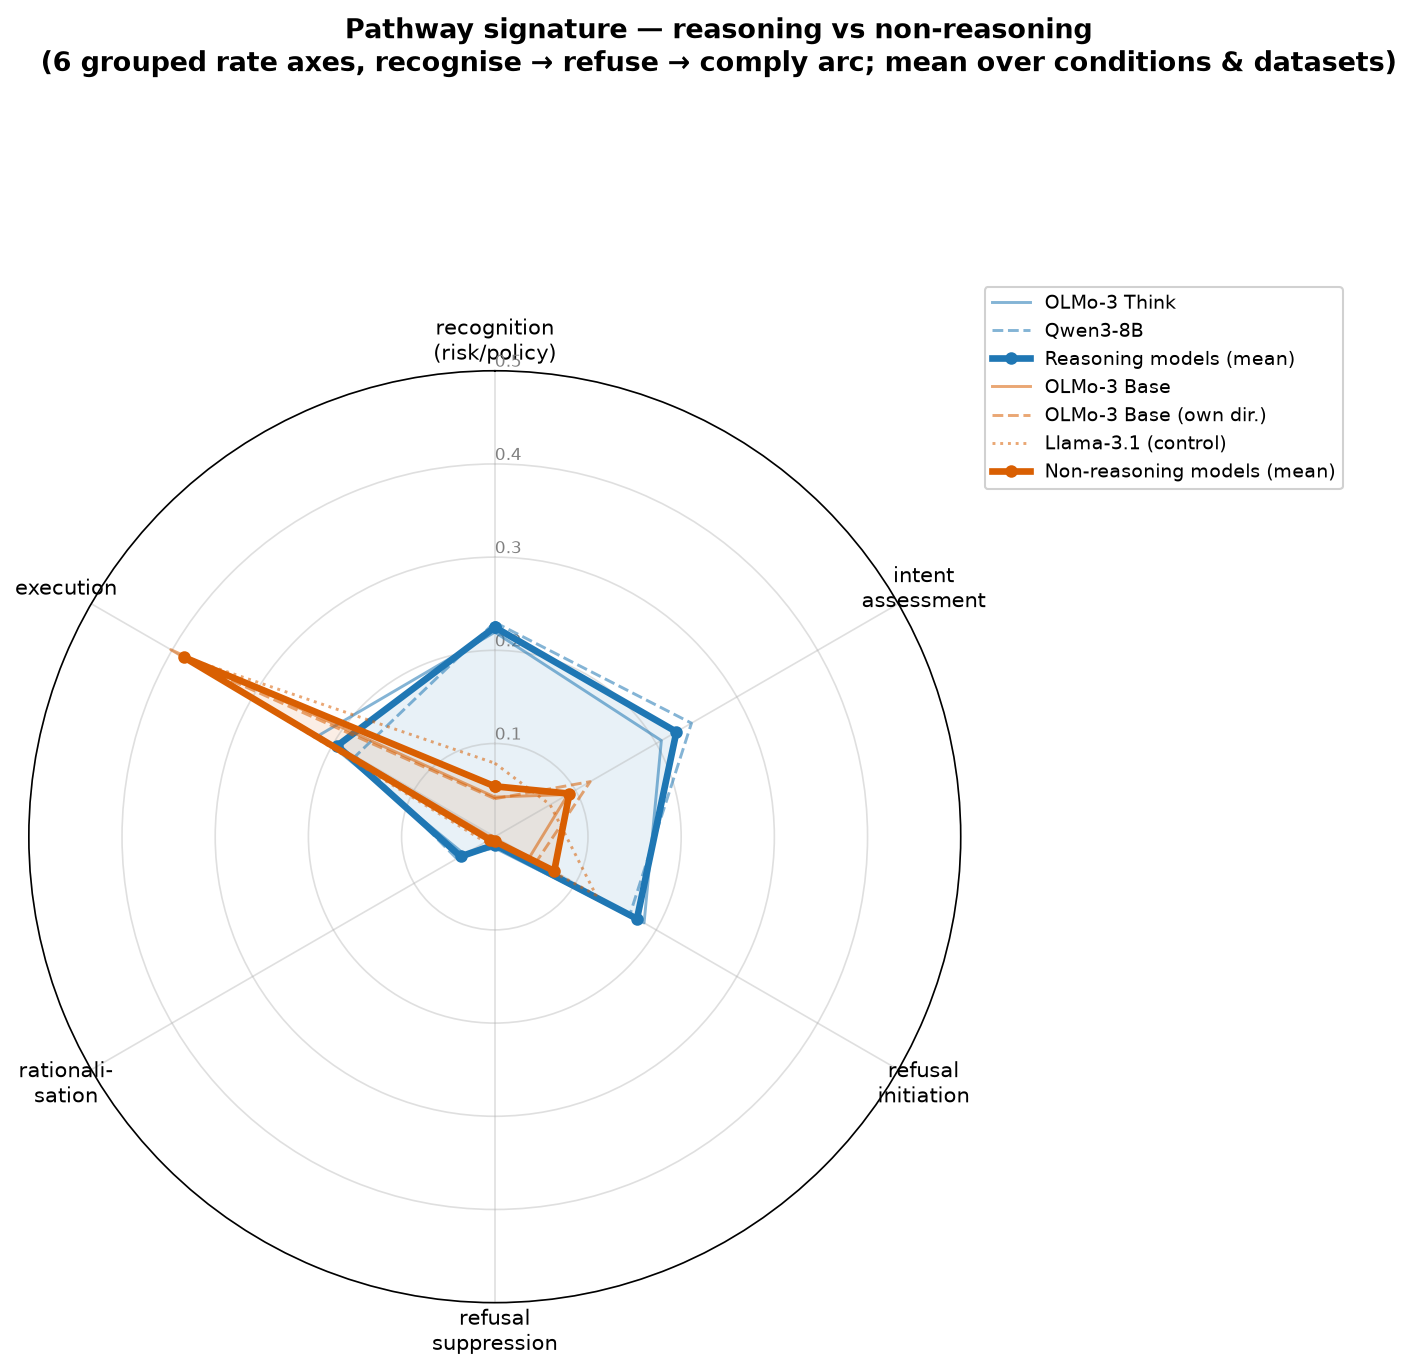
\includegraphics[width=\columnwidth]{figures/pathway_radar_reasoning.png}
  \caption{Pathway signature, reasoning vs non-reasoning models, on the six grouped
    axes (mean over conditions and datasets). The two classes trace opposite shapes:
    reasoning models keep recognition and refusal-initiation high and execution low;
    non-reasoning models do the reverse.}
  \label{fig:appendix-reasoning-radar}
\end{figure}


\end{document}
